% 来源：OEBPS/Text/Section0001_split_003.xhtml#sigil_toc_id_29

\BookChapter{19}
\section[第19章\q 加速财富积累第3招：减少费用，减少纳税]{第19章\\ 加速财富积累第3招：减少费用，减少纳税}

\begin{BookQuote}
把你口袋里的钱拿走，我们有的是办法。

\hfill ——建议美国国税局挂在墙上的格言
\end{BookQuote}

\begin{BookQuote}
你必须纳税，但是没有法律让你多付小费。

\hfill ——摩根士丹利公司的广告
\end{BookQuote}

现在你唱着摇滚——你正在奔向财务自由的大道上加速前进，因为你现在存的钱更多，赚的钱也更多了！还要做别的事吗？这些还不够吗？事实上，不够。你现在是内行了。你知道，最重要的不是你赚了多少钱，最重要的是你能留下来多少钱，装进你口袋里的才是你的钱。加速财富积累的第3招是，从你的投资中得到更多钱，办法是减少你的费用和税收，然后再把省下的这些费用和税款拿去做投资，这样你的投资更多，赚的钱自然也会更多。

还记得我们在第7章中提到的案例吗？3个从小玩到大的小伙伴，在35岁的时候，他们都投资了10万美元，投资收益率都是每年7\%，但是每个人承担的费用不同，分别是1\%、2\%、3\%。日积月累，复利效应造成了他们最终积累的财富相差几十万美元。泰勒付的费率只有1\%，杰森付的费率是3\%，但两个人积累的财富相差1倍。杰森的投资增值到574349美元，但是扣除费用之后真正拿到手的钱只有324340美元。

记住，公募基金这些隐藏的费率平均达到了3.17\%，简直高得离谱。那么持有一只高成本、高费率的公募基金，与持有一只低成本的指数基金相比，你多付的费用相当于你工作十年所积累的财富。这明显会拖累你奔向财务自由的前进速度。学术研究表明，那些收取很高费用的公募基金，其业绩几乎很少能跑赢市场平均水平。你付了很高的费用，已经受到了伤害，却连市场平均业绩水平也达不到，你又受到了侮辱。你可真惨。

\begin{figure}[htbp]
\centering
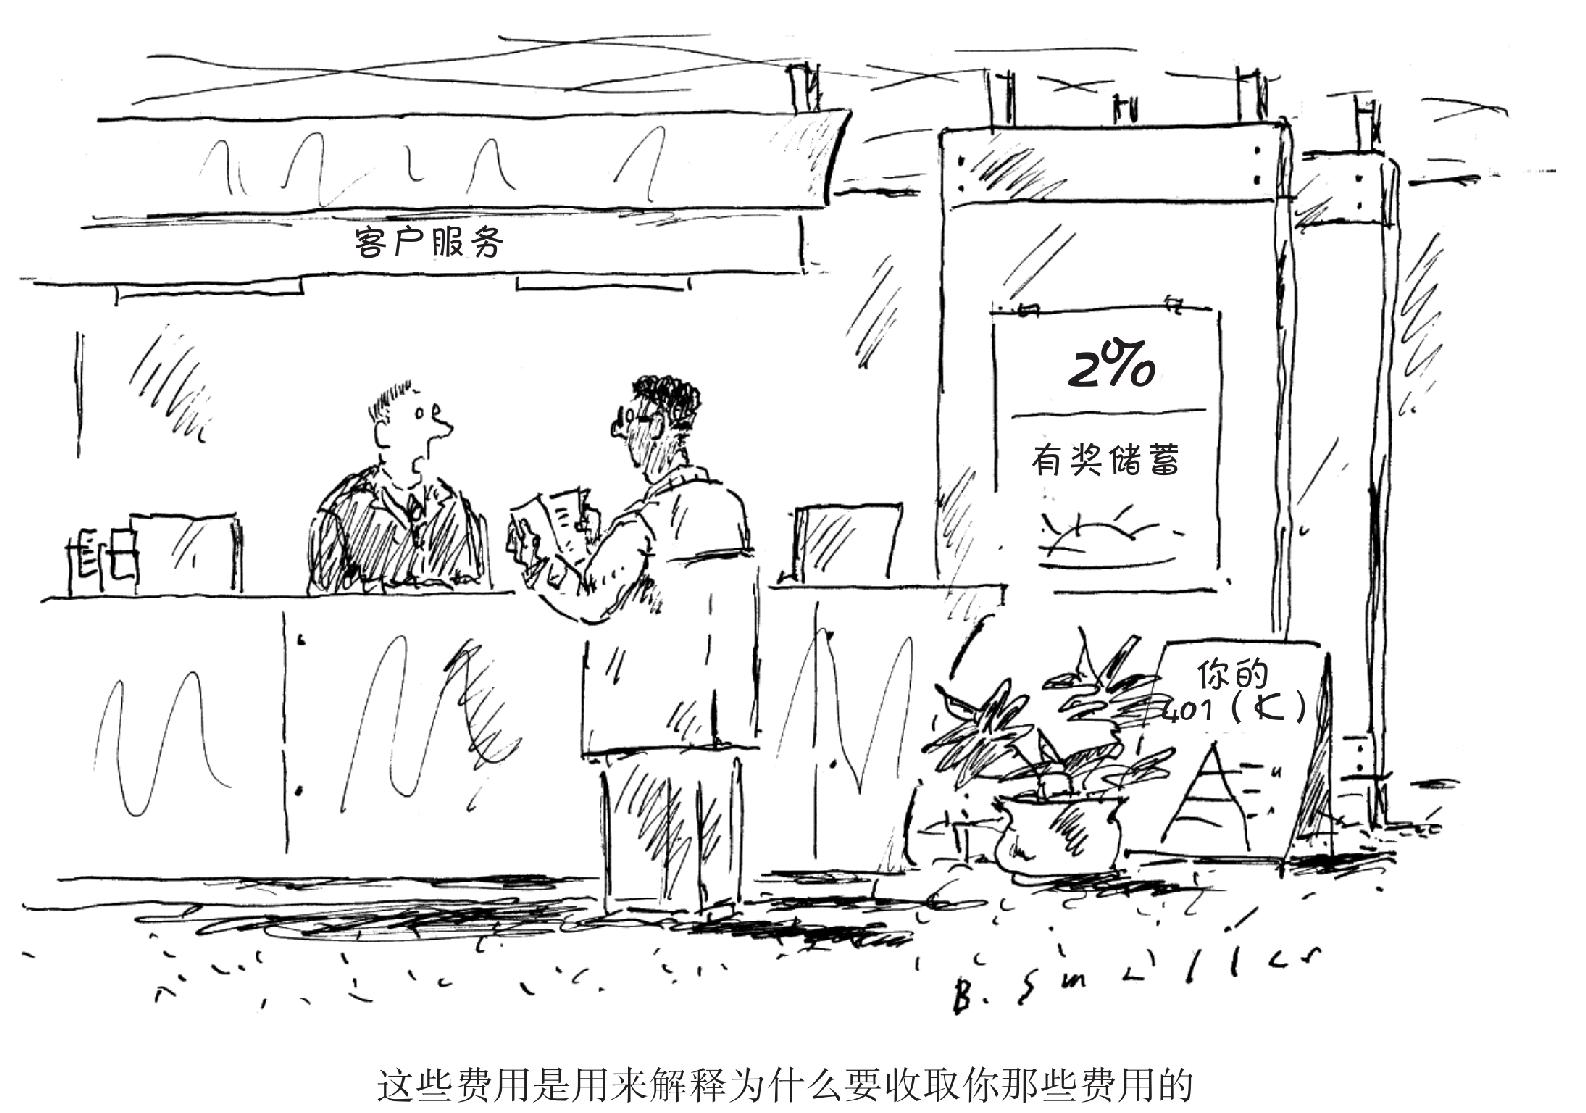
\includegraphics[width=0.80\linewidth,keepaspectratio]{image/19-1.jpg}
\caption{}\label{fig:19-1}
\end{figure}

所以，要远离那些过度征收的费用，兄弟姐妹们，快逃吧。找到低成本的指数基金来投资，一定要记住约翰·博格的警告，他向我们证明了支付过高的费用，会吃掉你未来投资收益的50\%\textasciitilde{}70\%。投资秘诀很简单：节省你的费用，用这些省下来的钱做投资，享受复利增长。节省费用这个策略是另一条通向财务自由的快车道。

和基金的费用相比，吞噬你储蓄更多的是什么？相关调查表明是税费。

在我们的生命历程里，平均而言，每个美国人要把自己收入的一半，甚至更多，拿来支付各种各样的税，比如所得税、财产税、销售税、加油税，等等。（按照很多专家的估计，现在美国人平均每一美元的收入，就要拿出54.25美分交税。）山姆大叔（美国政府），你好狠。别急，我还没有说完，让你花钱的还有费用。

税务局从你的收入中拿走54.25\%之后，你挣的每一美元还要再拿出来17.25\%来付贷款利息和基金费用。买车用车贷，买房用房贷，购物刷信用卡，上学用学生贷款，你花钱很方便，但你到处欠债。2014年美国平均每个家庭的信用卡债务超过1.5万美元，学生贷款超过3.3万美元，房产抵押贷款超过15万美元。从美国国家层面来看，美国人已经完全淹没在债务里了。

\begin{figure}[htbp]
\centering
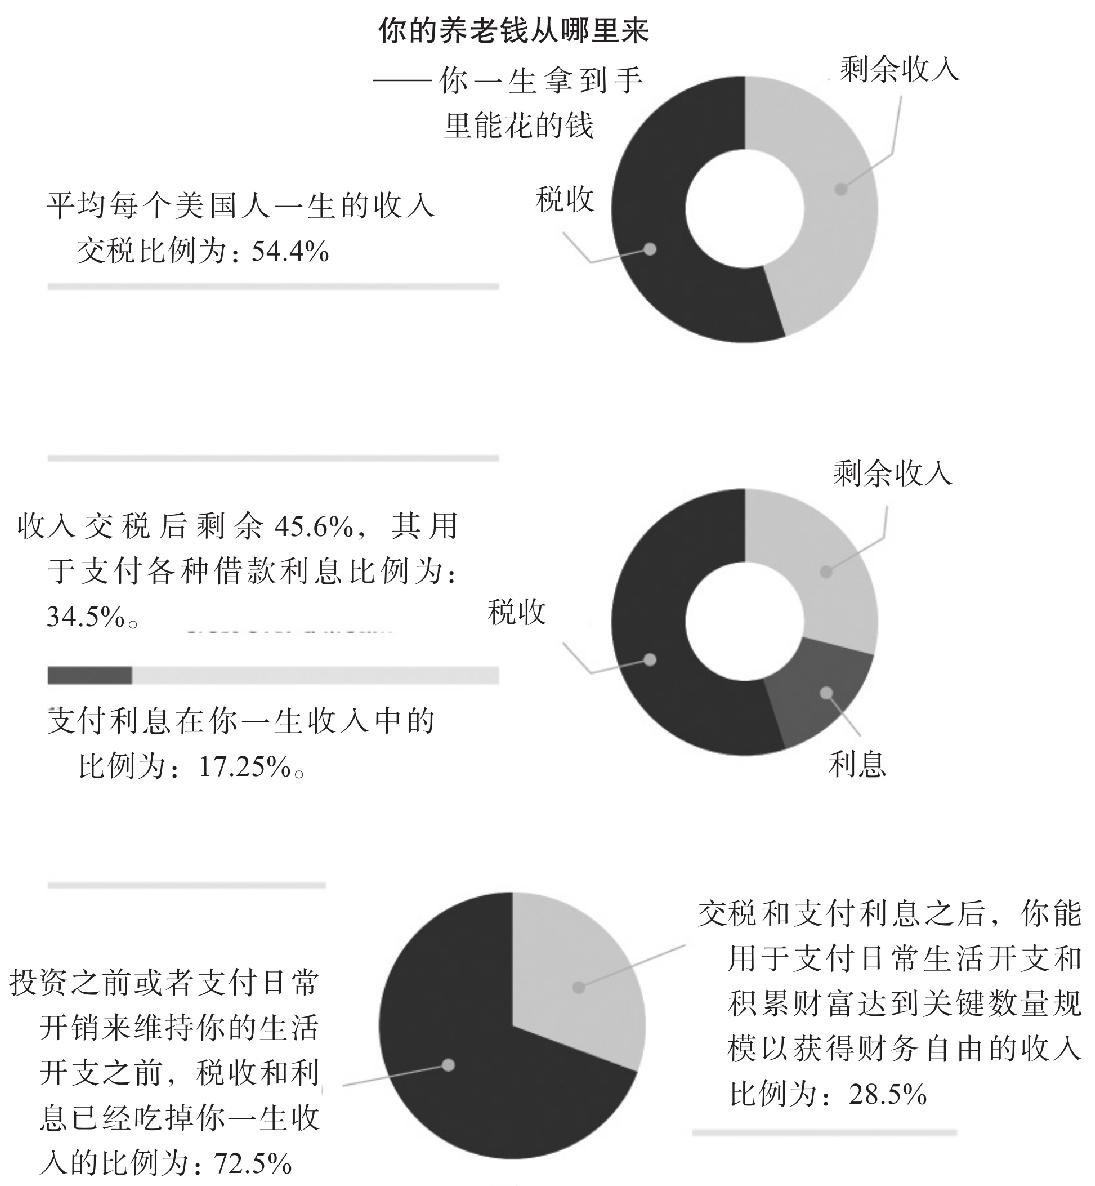
\includegraphics[width=0.65\linewidth,keepaspectratio]{image/19-2.jpg}
\caption{}\label{fig:19-2}
\end{figure}

事实上，平均而言，你的税后收入约有1/3会花在支付利息上。

这样纳税又支付利息之后，你辛辛苦苦挣的钱只剩下原来的28.5\%。你要用这笔钱支付生活中的其他各项开支：食物、衣服、教育、住房、健康医疗、旅行、娱乐，还有那些你在商场里或者亚马逊上看到的、一时冲动想要购买的各种东西！你还要找到办法，拿出来一些钱储蓄起来做投资，以积累财富，获得财务自由，或者至少是能让你退休后获得某种形式的稳定收入。

要把你的税收变得更加高效，你就要找到一种方法把你交出去的税（占你年收入的54\%）拿回来一些，让你辛辛苦苦赚的钱，能留在自己口袋里的更多一些。这些钱你可以拿去投资，实现复利增长，以更快地获得自己想要的财务自由。

事实上，如果你的年收入很高，而且住在一个所得税很高的地区，像加利福尼亚州（我过去就一直住在那里），那么你要交的所有税费（包括利息收入税、投资收益税、工资收入税等），加到一起会高达62\%。这意味着除非你有一个高效的节税策略，否则每挣到1美元，你只能留给自己0.38美元。

你有义务交纳你应该交的税，但你根本不必要多交一分钱的税。事实上，这是你作为一个公民的权利，只交该交的税款，此外不多交一分钱的税款。不要支付超过你需要支付的税款，正如比林斯·勒恩德·汉德——美国有史以来影响力很大的法官之一——所说的那样：

任何人都可以安排好自己的事务，好让自己交的税尽可能低。任何人没有义务非要选择那种给美国财政部交税最多的方式，甚至也根本不存在一种爱国的责任来增加人们的税款。美国最高法院一次又一次地说过，安排好自己的事务，让自己交纳尽可能低的税，这不邪恶。每个人都可以这样做，不管是富人还是穷人，所有人这样做都是对的，因为没有人有任何公共责任要多纳税——比法律规定的税还要多。

我觉得汉德大法官说的都是至理名言，照他说的做肯定没错。我认为，按照法律规定，我当然应该一分不少地足额纳税，但除此之外，我根本不应该再多交一分钱的税款，我觉得你也不应该多交一分钱的税款。我持续寻找合乎法律也合乎道德的方法来降低自己所交的税款，尽我最大的努力，充分利用政府的税收优惠政策，让我能在一个免税的环境下积累财富。我从很多投资大师那里学到的是，提高税收效率的意思是，交的税更少是一个最直接有效的办法，它可以缩短我们的致富路程，让我们从现在的财富水平更快地到达我们想要达到的财富水平。

\begin{BookQuote}
我很骄傲，我在美国向美国政府纳税。我同样骄傲的是，只交一半的税。

\hfill ——阿瑟·戈弗雷
\end{BookQuote}

我要先说清楚我是一个爱国者。我爱美国。我是“美国梦”的几百万个好榜样之一，而且我很高兴（也许应该说不是很高兴，而是很骄傲）交了我该交的税。我每年都要交好几百万美元的税款，我交的税款甚至比我以前梦到的钱还要多。但是我从戴维·斯文森那里知道，只有三种力量能够帮助你取得最高的投资回报：

1.资产配置

2.分散投资

3.税收效率

当然，戴维管理经营的是一个非营利组织，能够享受很多免税的优惠政策，这对他减少纳税很有帮助。但是对于我们大多数人来说，即使按照现在的税法，你也有办法让自己的投资收益最大化，让自己的纳税最小化。

\textbf{金钱威力法则4：}税收效率是最简单的方法之一，能够持续提高你的投资组合的真正收益率，即税后净收益率。税收效率越高，税后净收入越多，实现财务自由的速度越快。

（敬告读者：如果你一听我谈到纳税，你的脑子就犯糊涂，我很理解！请你马上停止阅读这一章，赶紧跳到下一章，好让你不会失去那股冲劲。但是，一定要安排一段时间，坐下来跟你的受托人投资顾问谈一谈，或者找个税收问题专家，学习了解如何让你的投资达到最高的税收效率。你如果愿意做这件事，接下来几页的内容提供了一些简单的减税、免税的好办法。如果能理解，你就能够留住自己大部分的投资收益，更快地实现你的财务梦想。）

\subsection{挑选你的税种}

如果你意识到，只要掌握一小部分纳税的知识，就能让你少交很多税，让你再也不是一个“税盲”——节省30\%的所得税，你会怎么办？少交这么多税，能让你实现财务目标的时间提前多少年？

作为投资者，你必须密切关注以下三类税收：

1.普通的收入所得税

如上所述，如果你属于高收入者，那么你的美国联邦所得税和州所得税加在一起要接近或超过50\%。

2.长期资本利得税

这个税适用于你持有时间超过一年之后才卖出的投资，按照投资收益来征税，税率只有20\%。

3.短期资本利得税

这个税适用于投资持有时间没有达到持有的最低年限——一年，按照投资收益来征收，现在这个税率和普通的收入所得税一样高，接近或超过50\%。我的天哪！

既然你已经知道了复利的力量，我敢肯定你也意识到了你的税率是50\%，和税率20\%相比，长期按复利积累下来，50\%的税率从你的投资收益中拿走的钱会更多，这导致你达到自己的财务目标的时间差别会很大。低税率可能让你提前十年达到你的财务目标，高税率可能让你永远无法达到你的财务目标。

想要了解不同税率的实际影响有多大吗？

\begin{itemize}
\item 如果你持有的公募基金总体投资收益率为8\%，你付的费率平均为3\%——让我们假设是2\%，保守一点儿估计。
\item 那么现在你8\%的收益减去2\%的费用之后，你的收益率是6\%。不过，别着急，还要扣税呢。
\item 如果你属于高收入者，住在加利福尼亚州或纽约州这样所得税相当高的地方，那么你要交的联邦所得税和州所得税加在一起要50\%。你扣费后6\%的投资收益，还要交50\%的所得税，这样再扣税后的投资净收益率只有近3\%。
\end{itemize}

记住，你能花的钱只能是你留到自己口袋里的钱。如果你的投资只能获得3\%的净收益率，那么你要花24年才能让你的投资翻倍。

如果你投资相同的金额，但是投资的基金不是主动管理型公募基金，而是被动管理型指数基金，你得到的也是8\%的投资收益率。但你交给基金公司的费率范围是10\textasciitilde{}50个基点，即0.1\%\textasciitilde{}0.5\%，我们用那个大一点的数字0.5\%来计算，只是为了保守一些。这意味着你的投资收益率8\%扣除费用之后，你还能得到每年7.5\%的扣费后的收益率。但是因为指数基金本身不经常买进、卖出股票，你可以递延交纳所有资本利得税，所以你扣税后的净收益率也是7.5\%。这意味着你可以把这些收益再投资，继续利用复利那不可思议的力量。

如果你小心谨慎地管理好你的投资，提高税收效率，并能够长期保持扣税后7.5\%的年化收益率，这样就能让你投资翻倍的时间只用9.6年，而不是24年。现在你看明白税收效率和费用效率的重要性有多大了吧？

如何降低你要交的税款，保留更大比例的投资收益，让你的投资能够更快地利用复利增长，从而更快地实现你的财务自由梦想？

\begin{itemize}
\item 你要确认不管在哪里，你投资用的方式能让你递延纳税［401(k)账户、个人退休金账户、年金、确定领取型计划］，好让你的投资利用复利增长得到的投资收益不用纳税，只有在你卖出投资的时候才要交税。或者创造一个未来免税的环境，办法是用罗斯账户来投资，这样以后所有的投资收益都能免于交税。
\item 如果你的投资不是在可以税收递延的账户里，也就是说不能享受递延纳税的优惠，那么在你卖出任何一笔投资之前，一定要确认这笔投资至少持有了一年零一天，以确保其符合更低长期资本利得税税率的要求（再说一下，当我写本书的时候，长期资本利得税税率是20\%）。
\end{itemize}

\subsection{还有一件事：小心公募基金}

对于大多数人来说，卖房这种事往往十年才发生一两次，你的会计师或者税收专家很容易向你解释明白如何做能够纳税最少。但是让我们来看一看公募基金，它有很大不同。你知道这些公募基金的基金经理每天都在做些什么？他们每天都在交易。他们买卖股票和债券，每天，每个月，每个季度，他们先买进，再卖出。证券行业称之为“周转”。买进卖出次数越多，投资组合周转率越高。

哥伦比亚广播公司（CBS）旗下市场观察网的查理·法雷尔的说法是：“尽管基金公司的市场营销材料都鼓励投资者要买入并长期持有。但是基金经理说的是一套，做的是另一套。他们真正的意思是，你要买入他们的基金并长期持有，而他们拿了你的钱之后，买了又卖，卖了又买，把你的退休金天天倒腾来倒腾去，像个疯子一样。”

专家说，大部分公募基金被买入后的持有时间都不满一整年。为什么你要买这种公募基金？难道你指望经理们这样的短线交易能够创造出更好的业绩吗？你知道这意味着什么？除非你持有这些基金是用你的401(k)账户，不然的话，基金经理的任何投资利得，一般都要让你来支付他们的收入所得税。\footnote{\label{fn:pdf-19-1}不过，在某种情况下，投资收益可能是长期的，因为基金已经拥有这些头寸一段时间了。}

简而言之，很大的可能是，你正在被征收35\%、45\%、50\%，甚至更高的个人收入所得税，这取决于你住在哪个州和你的收入水平。所有这些税都要由你来交，尽管你根本没有卖掉你的公募基金，没有实现投资收益。真冤！所以，你购买并持有公募基金，并不能保证你所有的资本利得，让它们继续按照复利增值，把所有税收递延到最后卖出基金的时候再交，你买这样频繁交易的股票基金，其实是你要为这些短期的资本利得交很高的所得税，给你的投资复利增值能力造成毁灭性的打击。如果你明白税收效率的话，这本来是可以避免的。

甚至如果你的401(k)和个人退休金账户缴费已经达到规模上限了，你还可以用另外一种方式来投资，而且能递延纳税。指数基金并不经常交易个股，它们一般会按照一个固定的股票篮子（即指数成分股）来长期持有这些公司的股票，唯一的变化就是这个指数基金追踪的指数调整了成分股——这种事情非常少见，一年一般一两次，而且一般只调整几只股票。

结果，如果你投资一只指数基金很长时间，那么你每年就不会被税收吞掉一大部分投资收益。相反，你能把税收递延到最后卖出的时候才交，因为你什么东西都没有卖出，没有实现任何投资收益，所以你不用交资本利得税了。这些投资收益能够一直留在基金里，持续按照复利增值，创造财富给基金的持有人——就是你！

你的受托人投资顾问或者一个税收专家，能够帮助你明白所有这些降低纳税的方法，让你的财务自由基金投资可以创造出更高的税后净收益，让你的复利增值过程的时间长度最大化。要知道，这能够节省你好多年甚至十多年的财富积累时间，让你更早地获得财务自由。

最后，再教你一个节税策略，你会在后面的内容中学到：这是经美国税务局批准的一种方法，可以让你大幅降低纳税额，因为这能让你的投资按复利增长，帮助你保留所有的投资收益，而且完全免税。这样做能让你更早地达到你的财务目标，比你原来预想要花费的时间提早1/4\textasciitilde{}1/2的时间，而且你根本不用为此多承担任何投资风险！

你是不是对我说的很有兴趣？我希望是。因为这是你的钱，这些钱决定着你的人生！不要让任何人拿走你的钱或者浪费你的钱！那么现在已经有了进入快车道的三条投资策略，它们能够加速你的财富积累速度，让你更快地赢得金钱游戏：

1.省的钱更多，把多省出来的这些钱做投资，这样你的投资本金更多。

2.赚的钱更多（为别人增加更多价值），把多赚的钱拿去投资，让你的投资本金更多。

3.减少费用和税收，把省下来的钱做投资，让你的投资本金更多。

现在你可以再加把油，快来看看，有一些方法可以进一步提高你的投资收益……
